\section{Risultati dello swing-up}
Adottando qualche accorgimento, il sistema riesce a eseguire lo swing-up.
Seguono tutte le considerazioni al riguardo.
% LQRegulatorGains[
% ssm /. params, {Q, R} /. {r11 -> .05, q11 -> 2} /. params]
% THIS is kinda what I used for the swing up.

\subsection{Simulazioni e parametri}
Considerando i parametri del motore, un limite conservativo
per la forza massima che questo può esercitare è
\begin{equation*}
    f_{\max} = 10N.
\end{equation*}
Approssimo l'accelerazione del carrello come
\begin{equation*}
    a \approx \frac f {M + m}
\end{equation*}
e trovo una stima per $a_{\max}$:
\begin{equation*}
    a_{\max} \approx \frac {f_{\max}}{m+M} \approx 40 \sfrac m {s^2}.
\end{equation*}
La simulazione in \autoref{fig:swingup-overflow} mostra che,
con questa scelta di parametri, il sistema
reale non raggiungerebbe
l'intervallo di controllabilità prima della fine della rotaia.
Dopotutto, la strategia che uso non tiene conto
in alcuno modo della variabile $q$.

\begin{figure}[h]
    \centering
    \begin{subfigure}[]{\textwidth}
        \centering
        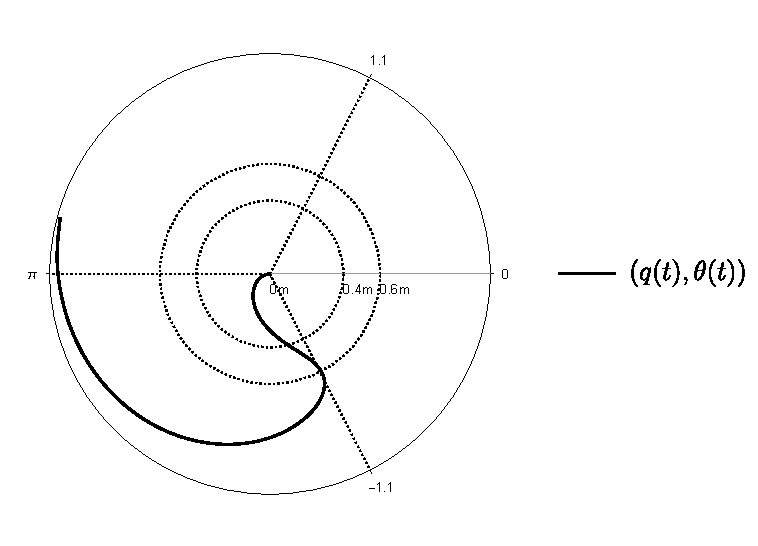
\includegraphics[width=.8\textwidth]{assets/polar-swingup-simulation}
    \end{subfigure}

    \caption[Simulazione swing-up fallito]{
        Simulazione di uno swing-up che non rientra nei limiti di lunghezza della
        rotaia. Il grafico è disegnato in coordinate polari.
        La coordinata radiale rappresenta la posizione del carrello $q$, in metri;
        la coordinata angolare rappresenta l'angolo del pendolo $\theta$.
        In questa simulazione il moto inizia dall'origine ed è contenuto
        per intero nella regione $q > 0$.
        Nel grafico è riportato il limite della rotaia ($.4m$), il limite
        di applicabilità di LQR ($1.1rad$) e il valore di $q$ per cui l'angolo
        rientra in questo limite ($.6m$).
    }
    \label{fig:swingup-overflow}
\end{figure}

Ho risolto questo problema adottando alcuni accorgimenti.
\begin{itemize}
    \item A parità di accelerazione, il motore trasferisce più
    energia al pendolo quando $|\theta| \approx \pi$.\footnotemark
    Ho quindi fissato un intervallo per $|\theta| > \theta_{\min} $ in cui il
    controllo è azzerato.

    \item Ho usato un valore di $a_{\max}$ più alto di quello
    stimato. L'effetto ottenuto è che il motore raggiunge la massima
    potenza più velocemente.

    \item Al posto di controllare il sistema verso $E = 0$,
    controllo il sistema verso un energia positiva $E = \Delta E$.
    In questo modo ho un piccolo margine per tenere conto di attriti
    e altri fattori non modellati.

    \item Ho usato una strategia di stabilizzazione più aggressiva,
    così da ridurre lo spazio che il carrello deve percorrere prima
    di tornare verso $q = 0$.
\end{itemize}

\footnotetext{Per convincersene, è sufficiente studiare l'andamento
della~\eqref{eq:dvdt} per un valore arbitrario di $\dot \theta \neq 0$.}
I parametri finali che ho usato per il sistema reale sono riportati
in \autoref{tab:parametri-swingup}

\bgroup
\renewcommand{\tabularxcolumn}[1]{>{\arraybackslash}m{#1}}
\renewcommand\arraystretch{1.5}
\begin{table}[H]
    \centering
\begin{tabular}{| gc | c | }
        \noalign{\hrule height 2pt}
        %todo°ò.-
        \rowcolor{Black}%
        \multicolumn{1}{=c}{\rowstyle{\bfseries\sffamily \color{White}} Parametro} & \multicolumn{1}{+c}{ Valore} \\
        \hline
        $q_{11}$ & $2$ \\
        \hline
        $r_{11}$ & $.05$ \\
        \hline
        $\Delta E$ & $.2 E[(0, 0, \pi, 0)^\T]$  \\
        \hline
        $\theta_{\min}$ & $2$ \\
        \hline
        $\theta_{\max}$ & $.6$ \\
        \hline
        $\dot \theta_{\max}$ & $6 s^{-1}$ \\
        \hline
        $a_{\max}$ & $77.6 \sfrac m {s^2}$ \\
        \hline
        \noalign{\hrule height 2pt}
    \end{tabular}
    \caption{Parametri per controllo combinato di swing-up e stabilizzazione.}
    \label{tab:parametri-swingup} %todo qui manca la descrizion2e di un tot di parametri.i
\end{table}
\egroup


\subsection{Comportamento del sistema}
Il sistema reale riesce ad eseguire lo swing-up.
In base alle caratteristiche del motore, si possono osservare due
comportamenti possibili:
\begin{enumerate}
    \item il pendolo viene portato in posizione verticale in un
    singolo movimento, oppure
    \item il pendolo viene fatto oscillare prima di raggiungere la
    posizione verticale.
\end{enumerate}
L'osservazione di uno dei due dipende
dalla forza massima che il motore riesce ad esercitare sul carrello.
Se la forza è abbastanza alta, il motore riesce a trasferire abbastanza energia
al pendolo in un solo movimento e si osserva il comportamento~(1).
Se la forza non è abbastanza alta, sono necessarie più oscillazioni
e si osserva il comportamento~(2).

Il sistema che ho costruito sviluppa entrambi questi comportamenti,
in base alle condizioni esterne\footnotemark .
Riporto in \autoref{fig:swingup-real-one} solamente i dati relativi al comportamento~(1), in quanto sono
sufficienti per mostrare la logica seguita dall'equazione~\eqref{eq:control-strategy-tanh}.
Una descrizione più dettagliata di tutti i possibili casi è disponibile in
%todo cite paper swingup

\footnotetext{La temperatura esterna influisce leggermente
sia sui parametri del motore, sia sugli attriti dei cuscinetti,
    cambiando i parametri del sistema.}

\begin{figure}
    \centering
    \begin{subfigure}[]{\textwidth}
        \centering
        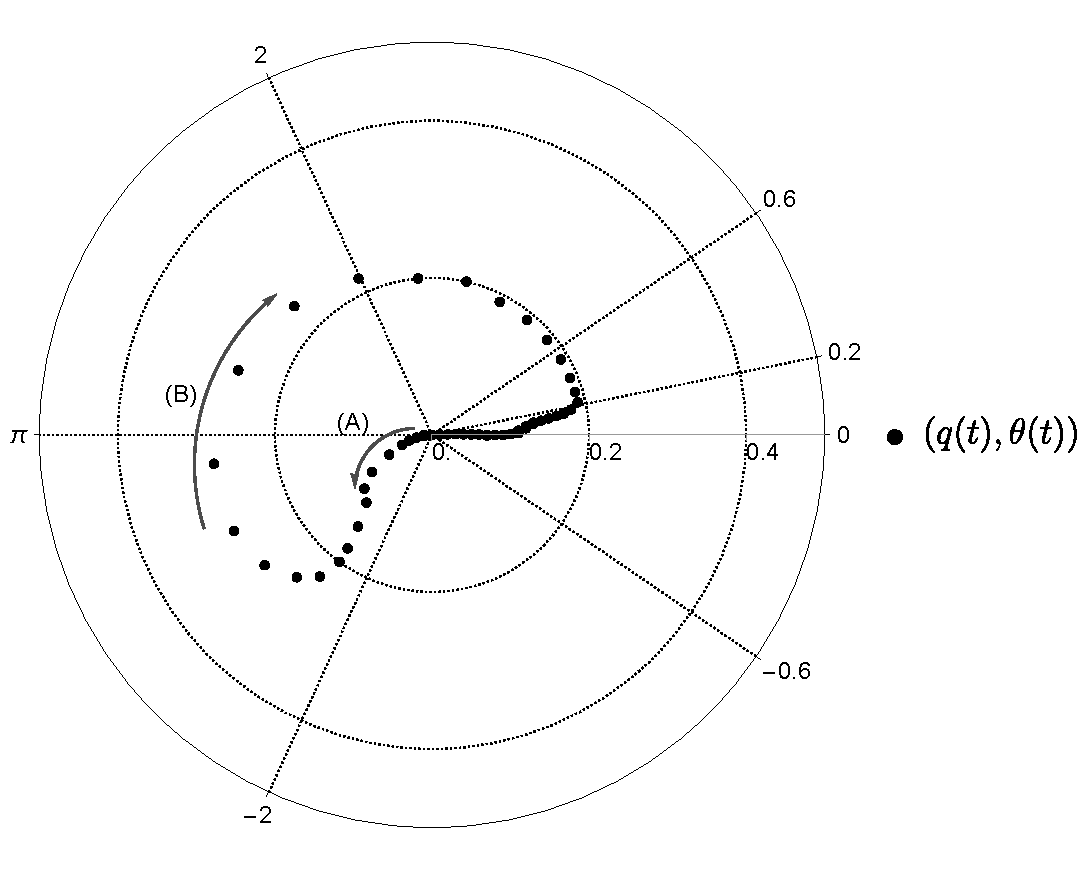
\includegraphics[width=.6\textwidth]{assets/polar-swingup-real}
        \caption{Posizione del carrello in funzione di angolo del pendolo.
        Il grafico è disegnato in coordinate polari ed è analogo
        al grafico in \autoref{fig:swingup-overflow}.
        Il moto inizia con un impulso esterno che sposta il pendolo
        verso sinistra (A). Il sistema risponde spostando il carrello verso
        destra (B). Il controllo è disattivato per $2 < \theta < .6$
        e rimane disattivato fino a $\theta = .2$, per via della velocità troppo
        elevata. Per $\theta < .2$ si attiva LQR e l'angolo e la posizione
        vengono riportati immediatamente a zero.
        }
        \label{fig:spazio-fasi-sistema-polare}
    \end{subfigure}
    \\[5ex]
    \begin{subfigure}[]{\textwidth}
        \centering
        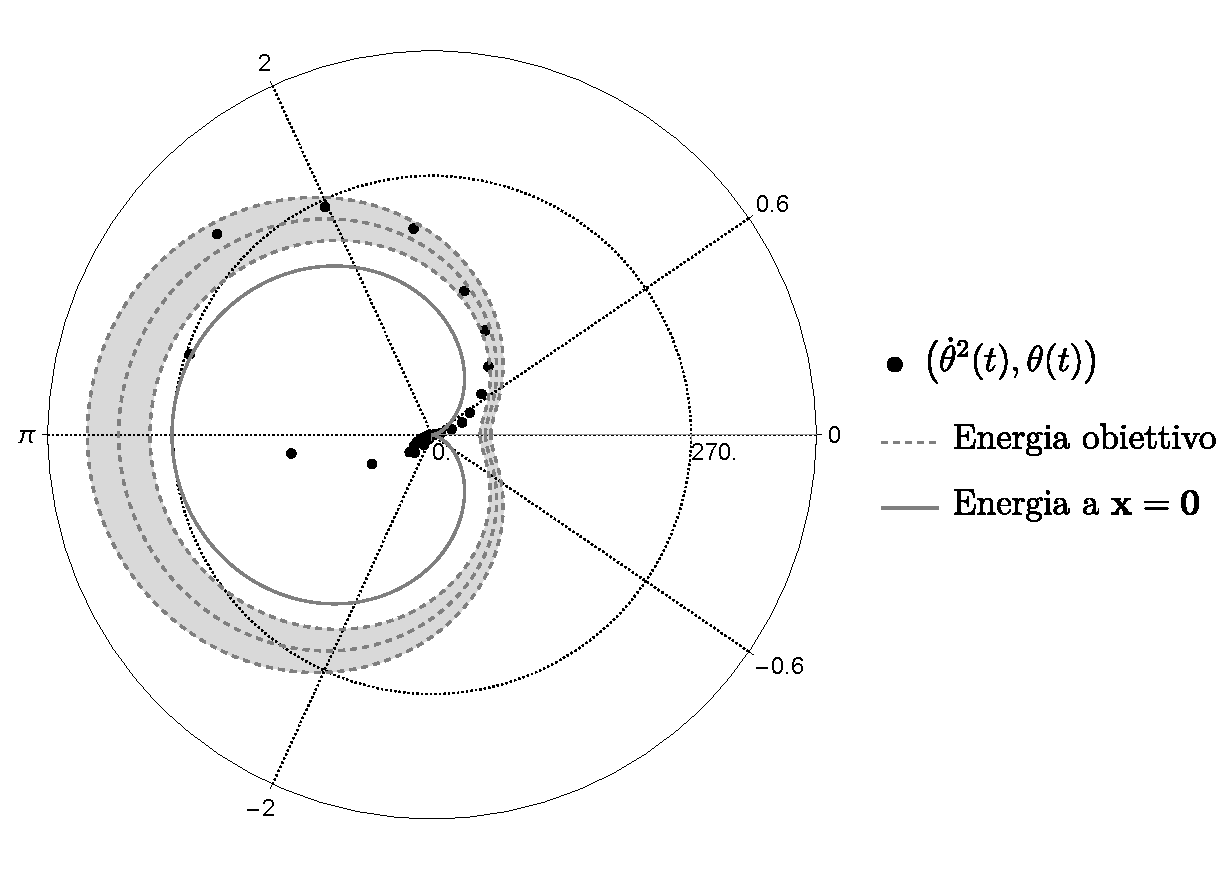
\includegraphics[width=.7\textwidth]{assets/polar-swingup-energy}
        \caption{
            Spazio delle fasi del solo pendolo, disegnato in coordinate polari.
            La coordinata radiale rappresenta il quadrato della velocità angolare
            del pendolo; la coordinata angolare ne rappresenta l'angolo.
            In questo spazio delle fasi, le curve a energia costante sono dei
            cardioidi. In figura, assieme ai dati sperimentali, sono
            mostrate le curve per $E=0$ e $E=\Delta E$, con un incertezza del
            $10\%$. Dalla figura si vede come l'effetto della strategia di swing-up
            è di posizionare il sistema nella traiettoria corrispondente 
            all'energia desiderata.
            Per $\theta < 2$ l'attrito sposta il sistema su traiettorie di
            energia decrescente e per $\theta < .6$ si attiva LQR che porta
            immediatamente l'energia a zero.
            
            %todo footnote per cardioidi
            %todo(non qui) footnote per equazione riccati
        }
        \label{fig:spazio-fasi-pendolo-polare}
    \end{subfigure}

    \caption[Dati di una procedura di swing-up]{
        Dati relativi ad una procedura di swing-up. Il grafico
        \ref{fig:spazio-fasi-sistema-polare} rappresenta un sottospazio dello
        spazio delle fasi dell'intero sistema. Il grafico
        \ref{fig:spazio-fasi-pendolo-polare} rappresenta lo spazio delle fasi del
        solo pendolo.
    }
    \label{fig:swingup-real-one}
\end{figure}


\todo{add proper figure description}

